\documentclass{beamer}

\usepackage{ctex}
\usepackage{graphicx}
\usepackage{amsmath}
\usepackage{amsfonts,amssymb}
\usepackage{algorithm}
\usepackage{algpseudocode}
\usepackage[export]{adjustbox}
\usepackage{subcaption}
\usepackage{tikz}
\usepackage{url}

\graphicspath{{./img/}}

\title{利用GSL求解方程$f(x)=0$的探索}
\subtitle{期末作业}
\author{张立言\\数学与应用数学\\3210101207}
\institute{浙江大学数学科学学院}
\date{2022年7月4日}

\begin{document}

\frame{\titlepage}

\begin{frame}
\frametitle{简介}
\begin{itemize}
\item 二分法适用于连续函数是一种方程式根的近似值求法。它是基于连续函数的介值性质以及实数的闭区间套定理推导出来。我们在下面也会尝试一种基于二分法的迭代方法Brent方法(Brent's method),这种方法相比于简单的二分法收敛更快。
\item 牛顿迭代(Newton's method)又称为牛顿-拉佛森方法(Newton-Raphson method),它是一种在y实数域和复数域上近似求解方程的方法。方法使用函数$f(x)$的泰勒级数的前面几项来寻找方程$f(x)=0$的根。
\end{itemize}
\end{frame}

\begin{frame}
\frametitle{数学理论}

有关二分法和牛顿法的收敛效果,我们可以由如下的一些定理进行描述:

\textbf{Theorem 1}{} 二分法达到精度$\varepsilon$,需要的最大迭代次数$N$满足:
\begin{equation}
  N \ge \frac{ln(b_0-a_0)-ln(\varepsilon)}{ln(2)}
\end{equation}

因为$\varepsilon$在对数下,当$\varepsilon$很小的时候,需要的迭代次数会急剧增大。
\end{frame}

\begin{frame}
\frametitle{数学理论}
\textbf{Theorem 2}{} 对于牛顿迭代法,有:
\begin{equation}
   \lim_{k \to \infty} \frac{e_{k+1}}{e_k^2} = |f''(\xi)|
\end{equation}
在这里,$e_k$表示第k次迭代的误差。\par
由上面的定理我们可以发现,牛顿迭代法的误差会以指数上的指数的级别缩小。所以说牛顿迭代法具有更好的收敛效果。\par
\end{frame}
\begin{frame}
\frametitle{数学理论}
\textbf{Theorem 3}{} 对于斜截法,有:
\begin{equation}
   \lim_{k \to \infty} \frac{e_{k+1}}{e_k^{\alpha}} = |f''(\xi)|
\end{equation}\par
这里$\alpha=\frac{1+\sqrt{5}}{2}$
通过简单的计算,我们知道$\alpha < 2$,这一点说明了斜截法相对于牛顿迭代,收敛效果较差。但是斜截法也有优点,它适用于于导数难以计算或者导数未知的方程求解,但是牛顿法对此无能为力。
\end{frame}

\begin{frame}
\frametitle{实验说明}
从Figure 1中我们可以看到,二分法以下界作为根的近似值。牛顿迭代法只需要4次即可达到迭代停止条件。

以不需要导数的迭代为例,我们可以采用布伦特方法。与牛顿迭代法进行比较,得到图像Figure 2.

Brent比起二分法,迭代次数大大减少。但牛顿法迭代次数仍然少于Brent方法。牛顿法有着更明显的优势。

我们再比较一下Newton method和斜截法。整理运行的数据得到Figure 3.从Figure 3中我们可以看到,牛顿法的收敛速度明显快于斜截法。
\begin{figure}[H]
  \begin{subfigure}{0.3\linewidth}
  \centering
  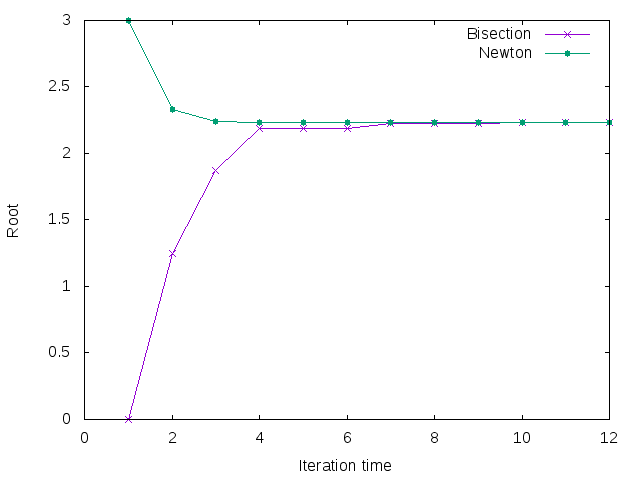
\includegraphics[width=1\textwidth]{graph1.png}
  \caption{Figure 1}
  \label{fig:1}
  \end{subfigure}
  \begin{subfigure}{0.3\linewidth}
  \centering
  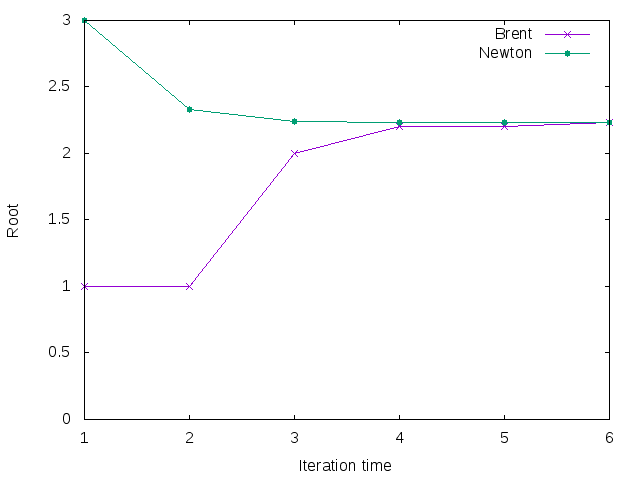
\includegraphics[width=1\textwidth]{graph2.png}
  \caption{Figure 2}
  \label{fig:2}
  \end{subfigure}
  \begin{subfigure}{0.3\linewidth}
  \centering
  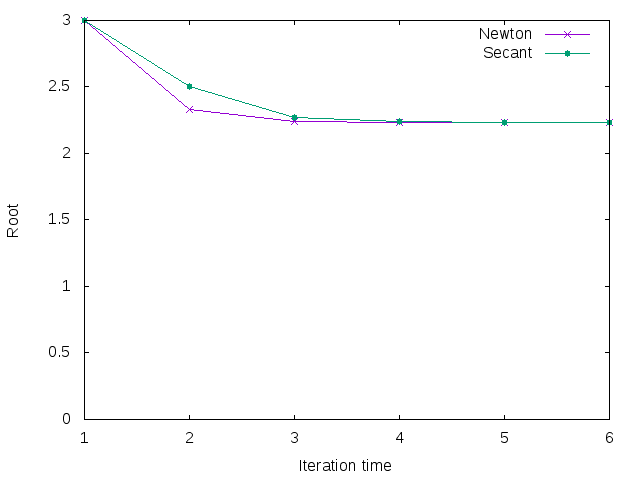
\includegraphics[width=1\textwidth]{graph3.png}
  \caption{Figure 3}
  \label{fig:3}
  \end{subfigure}
\end{figure}
\end{frame}

\begin{frame}
\frametitle{实验说明}
我们使用二分法和牛顿法解一个简单的超越方程:$f(x)=e^x-4x=0$.
我们确定根的区间为$[0,3]$,观察最终解的位置。
\begin{figure}[H]
  \begin{subfigure}{0.2\linewidth}
  \centering
  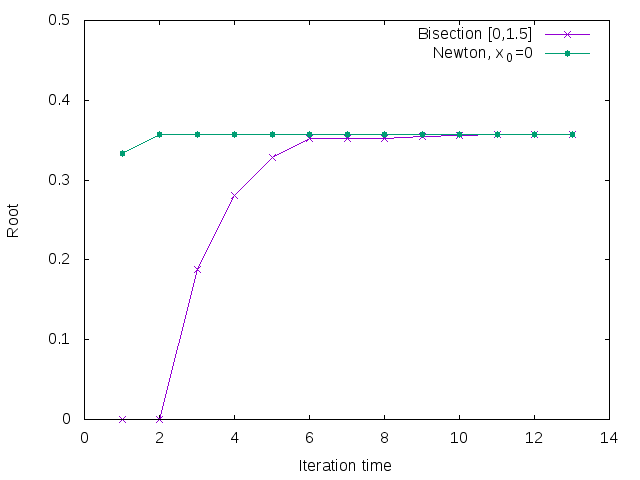
\includegraphics[width=1\textwidth]{graph4.png}
  \end{subfigure}
  \begin{subfigure}{0.2\linewidth}
  \centering
  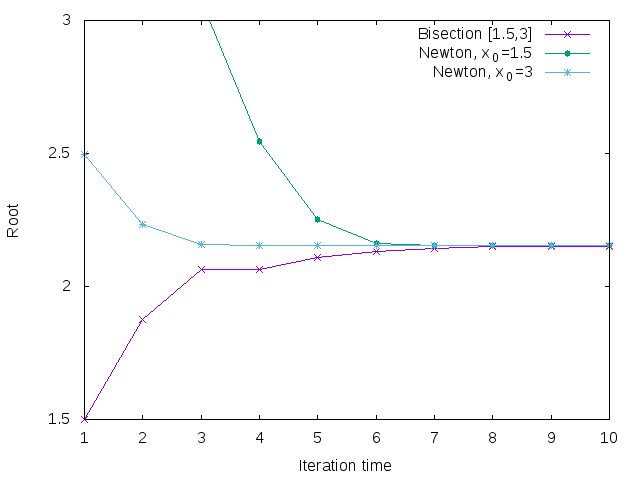
\includegraphics[width=1\textwidth]{graph5.png}
  \end{subfigure}
  \caption{Different initial values, and bisection}
\end{figure}

首先让牛顿迭代的初值分别为0,1.5和3,最终都收敛到了较大的根,由图中可以观察到,选取初值$x_0=3$的时候,收敛的速度跟快。二分法由于区间的限制,必定收敛于某一个大根或者小根,相比于两次牛顿迭代,二分法仍然没有优势。
\end{frame}

\begin{frame}
\frametitle{总结}
这次实验充分利用了GSL来进行科学计算,同时也让我们看到了不同的算法求解同一个问题,虽然理论上的最终结果都是相同的,但是由于计算机只能处理离散的数据,我们要尽可能的通过离散的数据处理去接近精确的数学理论,这就体现出了不同算法的相对优势。
\end{frame}


\end{document}
